\documentclass{article}
\usepackage{graphicx}
\usepackage{tikz}
\usepackage{lscape}
\usepackage[margin=2cm]{geometry}

\graphicspath{ {imágenes/Diagramas de flujo} }

\title{PROYECTO INTÉRPRETE ARITMÉTICO \\ Análisis y Diseño de Algoritmos \\ Universidad Panamericana}

\author{Ain Bolaños Cortés\\Esteban Eguiarte Maldonado\\Mariana Sánchez Esparza}
\date{Septiembre 2023}

\begin{document}

\maketitle

\section{Descripción y Análisis del Problema}
El siguiente programa tiene como objetivo resolver operaciones aritméticas básicas en las cuales el usuario solo podrá utilizar la suma y el producto. El usuario debe ingresar la operación aritmética válida expresada en una cadena de texto, en la que se permiten paréntesis, el signo de suma (+), el signo de multiplicación (*), números enteros y números decimales. Es importante destacar que no se pueden utilizar paréntesis para expresar el producto.\\

Uno de los problemas que hemos considerado como equipo es la posibilidad de que se ingresen caracteres no válidos, como letras o signos diferentes a la suma y el producto. Además, hemos tenido en cuenta otros problemas potenciales, como la inserción de dobles puntos decimales, paréntesis que se abren pero no se cierran, paréntesis vacíos y la posibilidad de que no haya suficientes operandos u operadores.\\


\section{Descripción de la Solución Propuesta}
La solución propuesta para abordar el problema se basa en una serie de funciones que trabajan en conjunto para resolver operaciones aritméticas a partir de una cadena de texto ingresada por el usuario.\\

Primero, la función \texttt{juntar} se encarga de eliminar espacios innecesarios y validar la entrada, asegurando que solo se trabaje con caracteres válidos. A continuación, se tiene la función \texttt{calcular}, que permite implementar recursividad para reducir cada expresión aritmética a expresiones mucho más simples y operables. Esta función comienza por utilizar \texttt{eliminar_parentesis}, que elimina paréntesis redundantes y simplifica la expresión. Luego, \texttt{num_valido} verifica si los números presentes en la cadena son válidos, evitando problemas como múltiples puntos decimales o caracteres no numéricos.\\

La función \texttt{encontrar_operador} busca operadores en la cadena, asegurándose de que haya suficientes operandos para realizar operaciones válidas. Esto se logra con la ayuda de \texttt{validar_par}, que se utiliza para encontrar el paréntesis que cierra el inicialmente identificado. Si se encuentra un operador, se llama a la función \texttt{calcular} para realizar los cálculos necesarios.\\

Finalmente, la función \texttt{main} sirve como punto de entrada del programa, donde se recibe la cadena del usuario, se procesa a través de todas las funciones mencionadas y se presenta el resultado. Esta solución proporciona una herramienta completa y precisa para resolver operaciones aritméticas básicas a partir de una interfaz de texto, garantizando la validación de la entrada y el cumplimiento de las reglas de precedencia en las operaciones.\\


\section{Algoritmos}
En esta sección se presentará un algoritmo por cada función hecha, cada uno se presentará en el orden según aparezca en el código principal.

\subsection{Algoritmo correspondiente a \texttt{function(juntar)}}
\begin{enumerate}
    \item Inicializar una cadena vacía llamada \texttt{nueva} que contendrá la cadena final.

    \item Obtener la longitud de la cadena de entrada y asignarla a la variable \texttt{n}.

    \item Iniciar un bucle que recorrerá cada caracter de la cadena de entrada desde el priemro hasta el último. Utilizaremos una variable llamada \texttt{ind} para llevar un seguimiento de la posición actual. 

    \item Asignar el caracter en la posición \texttt{ind} de la cadena de entrada a la variable \texttt{char}.

    \item Comprobar si \texttt{char} no es un espacio, un salto de línea o un tabulador para determinar si debe incluirse en la cadena \texttt{char}. Usaremos los caracteres correspondientes en Julia \texttt{('', '\t' y \'n')}

    \item Concatenar los caracteres que cumplan con la condición de la cadena \texttt{nueva}.

    \item Después de recorrer todos los caracteres, devolver la cadena \texttt{nueva} como resultado.\\
\end{enumerate}

\subsection{Algoritmo correspondiente a \texttt{function(num\textunderscore valido)}}
\begin{enumerate}
    \item Inicializamos una variable llamada \texttt{cuenta} con el valor 0. Esta variable se utiliza para verificar si un número contiene más de un punto decimal. 

    \item Asignamos la longitud de la cadena a la variable \texttt{n}.

    \item Iteramos a través de cada caracter de la cadena, comenzando desde el primero hasta el último, para verificar si son números, operadores válidos o puntos decimales. Utilizaremos la variable \texttt{ind} para recorrer los caracteres. 

    \item Asignamos el caracter en la posición \texttt{ind} de la cadena a la variable \texttt{char}.

    \item Comprobamos si \texttt{char} es una cifra, un operador o un punto decimal. Si ninguno de estos casos se cumple, se considera un error ya que no es una entrada válida para operaciones. 

    \item Si se encuentra un punto decimal, incrementamos la variable \texttt{cuenta} en uno. Al verificar todos los caracteres, si \texttt{cuenta} supera 1, se considera un error, ya que un número no puede tener más de un punto decimal. 

    \item La función debe devolver la entrada siempre y cuando sea un número válido.\\
\end{enumerate}

\subsection{Algortimo correspondiente a \texttt{function(eliminar\textunderscore parentesis)}}
\begin{enumerate}
    \item Asignamos la longitud de la cadena a la variable \texttt{n}.

    \item Si la longitud es 0, se considera un error, ya que hay un paréntesis vacío. Esto puede ocurrir cuando la función \texttt{calcular} llama a esta función y la cadena comienza con un paréntesis.

    \item Si lo anterior no se cumple y el primer caracter es un parentesis, llamamos a la función \texttt{validar\textunderscore par} para determinar el índice del paréntesis que cierra el paréntesis inicial. El resultado se asigna a la variable \texttt{ind\textunderscore final}.

    \item Si \texttt{ind\textunderscore final} es igual al último índice, significa que el primer  el último paréntesis son redundantes, por lo que devolvemos la cadena de texto desde el segundo caracter hasta el penúltimo caracter. De esta mandera, eliminamos los paréntesis redundantes. 

    \item Llamamos recursivamente a la función \texttt{eliminar\textunderscore parentesis} en el resultado final, ya que no hay paréntesis redundantes en ese punto. El resultado se asigna a la variable \texttt{texto}.

    \item La función devuelve la variable \texttt{texto} ya que no hay paréntesis redundantes en la cadena original.\\
\end{enumerate}

\subsection{Algoritmo correspondiente a \texttt{function(validar\textunderscore par)}}
\begin{enumerate}
    \item Inicializamos la variable \texttt{ind} con el valor 2. Esta variable se utilizará para iterar y comparar todos los caracteres, comenzando desde el segundo caracter, ya que el primero se sabe que es un paréntesis. 

    \item Asignamos la longitud de la cadena a la variable \texttt{n}.

    \item Iniciamos un contador que servirá para mantener un seguimiento de la cantidad de paréntesis abiertos. El contador comienza en uno, y se incrementa en uno cuando se encuentra un paréntesis abierto, y se resta uno cuando se encuentra un paréntesus cerrado.

    \item Mientras el índice sea menor o igual al último, realizamos comparaziones para verificar si los paréntesis están completamente emparejados. 

    \item Asignamos el valor del caracter actual a la variable \texttt{char}, y el valor del caracter anterior se asigna a la variable \texttt{char\textunderscore anterior}.

    \item Si el caracter actual es un paréntesis abierto y el caracter anterior pertenece a \texttt{cifras}, se considera un error, ya que no se puede multiplicar con un paréntesis, Lo mismo ocurre si después de un paréntesis cerrado, hay otro paréntesis abierto. Al final, se sumo uno al contador para indicar que se ha encontrado un paréntesis abierto. 

    \item Si el caracter actual es un paréntesis cerrado y el caracter inmediatamente anterior es un paréntesis abierto o un operador, se considera un error. No puede haber paréntesis vacíos ni operadores junto a un paréntesis cerrado. Además, si el caracter siguiente pertenece a \texttt{cifras}, también se considera un error, ya que no se puede multiplicar con un paréntesis. 

    \item Restamos uno al contador por encontrar un paréntesis cerrado. 

    \item Si el contador llega a ser 0 y hemos llegado al último caracter, retornamos el valor actual del índice. 

    \item Si el caracter siguiente inmediato no es un paréntesis cerrado, también retornamos \texttt{ind} para continuacr la comparación. 

    \item Al finalizar la revisión, sumamos uno al índice para continuar la comparación y repetir el proceso. 

    \item Si el contador es diferente de 0 después de revisar todos los caracteres, se considera un error.\\
\end{enumerate}

\subsection{Algoritmo correspondiente a \texttt{function(encontrar\textunderscore operador)}}
\begin{enumerate}
    \item Recibe dos argumentos: el caracter y la cadena. 

    \item Inicializa la variable \texttt{i} con el valor 1, que represetará el índice del caracter que se va a revisar y ayudará a verificar si se cumple la condición. 

    \item Asigna a la variable \texttt{n} la cantidad de caracteres en la cadena. 

    \item Mientras el caracter actual sea menor o igual al último caracter, se utiliza para separar paréntesis y encontrar operadores.

    \item Asigna a la variable \texttt{char\textunderscore act} el caracter actual.

    \item Si el caracter actual es un paréntesis abierto, actualiza la variable \texttt{i} con el índice del paréntesisi que cierra ese paréntesis. Este resultado proviene de la función \texttt{validar\textunderscore par}.

    \item Si el valor de \texttt{char\textunderscore act} es igual al caracter que recibió la función del inicio, la función debe devolver la posición en la que se encuentra. Esto ocurre cuando se encuentra un operador. 

    \item Si no se cumple la condición anterior, la función devuelve 0, ya que la posición 0 no es válida y continuará buscando el siguiente operador.\\
\end{enumerate}

\subsection{Algoritmo correspondiente a \texttt{function(calcular)}}
\begin{enumerate}
    \item Recibimos la cadena como entrada.

    \item Asignamos a la variable \texttt{n} la cantidad de caracterers en la cadena. 

    \item Si el primer caracter de la cadena es un paréntesis abierto, actualizamos la variable \texttt{texto} con el resultado de la función \texttt{eliminar\textunderscore parentesis}.

    \item Ejecutamos la función \texttt{num\textunderscore valido}. Si el resultado de la función es verdadero, entonces es un número válido y podemos aplicar la función \texttt{parsec} para leer el número. 

    \item Si no es un número válido, significa que hemos encontrado un operador, por lo que ejecutamos la función \texttt{encontrar\textunderscore operador}, que inicialmente busca el operador de suma.

    \item Si la función \texttt{encontrar\textunderscore operador} indica que el operador está en la primera posición (índice 1), es un error, ya que no hay operadores suficientes.

    \item Si el operador no está en la priemra posición pero sí en la última, también es un error, porque falta el último operador.

    \item Si el índice no es igual a 1, entonces hay suficientes operandos, por lo que procedemos a separar y llamamos nuevamente a la función \texttt{calcular} de manera recursiva para buscar más operadores o eliminar paréntesis.

    \item Si la función \texttt{encontrar\textunderscore operador} devuelve el valor 0, que no existe, significa que no se encontró el operador de suma. En este punto, la función buscará el operador de multiplicación. 

    \item Ejecutamos nuevamente la función \texttt{encontrar\textunderscore operador}, pero esta vez, buscamos el operador de multiplicación. 

    \item Si la función \texttt{encontrar\textunderscore operador} indica que el operador está en la primera posición (índice 1), es un error, ya que no hay operandos suficientes. 

    \item Si el operador no está en la primera posición pero sí en la última también es un error porque falta el último operador. 

    \item Si el índice no es igual a 1, entonces hay suficientes operandos, por lo que procedemos a separar y llamamos nuevamente a la función \texttt{calcular} de manera recursiva para buscar más operadores o eliminar paréntesis. 

    \item Ahora que todo está separado, podemos realizar las operaciones primero en los paréntesis, luego en el producto y finalmente en la suma.\\
\end{enumerate}

\subsection{Algoritmo correspondiente a \texttt{function(main)}}
\begin{enumerate}
    \item Creamos una variable \texttt{fin} con el valor \texttt{true}.

    \item Creamos una cadena vacía llamada \texttt{entrada} para recibir la cadea del usuario.

    \item Solicitamos al usuario que ingrese una cadena y proporcionamos onstrucciones sobre cómo funciona el programa.

    \item Utilizamos un bucle \texttt{while} para leer la cadena ingresada por el usuario.

    \item Usamos el comando \texttt{readline} para capturar la entrada del usuario y concatenarla a la variable \texttt{entrada}, que inicialmente estaba vacía. Continuamos concatenando elementos hasta que la cadena ingresada por el usuario esté vacía.

    \item Actualizamos la variable \texttt{fin} a \texttt{false} para interrumpir el ciclo \texttt{while}.

    \item Aplicamos la función \texttt{juntar} a la cadena ingresada. 

    \item Si el resultado después de aplicar \texttt{juntar} es una cadena vacía, se produce un error, ya que se entregó una cadena vacía.

    \item Mostramos el resultado de la función \texttt{calcular}.\\
\end{enumerate}

\section{Diagramas de Flujo}
En esta sección se presentará un diagrama de flujo por cada función hecha, cada uno se presentará en el orden según aparezca en el código principal.

\subsection{Diagrama de flujo correspondiente a \texttt{function(juntar)}}\\
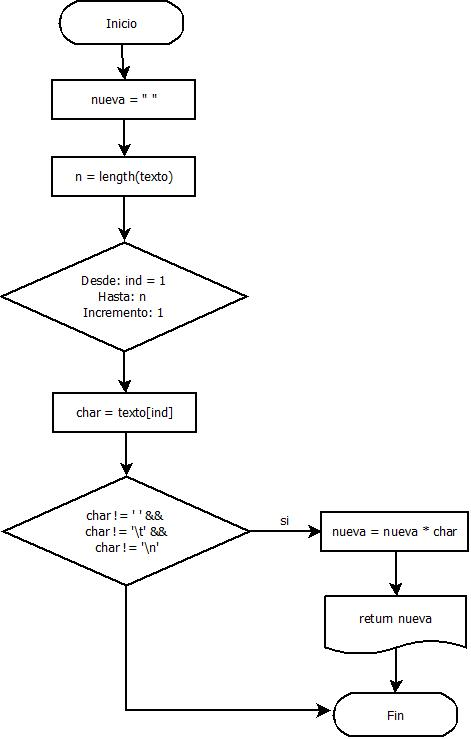
\includegraphics[scale=1]{Diagrama1.jpeg}

\begin{landscape}
    \subsection{Diagrama de flujo correspondiente a \texttt{function(num\textunderscore valido)}}\\
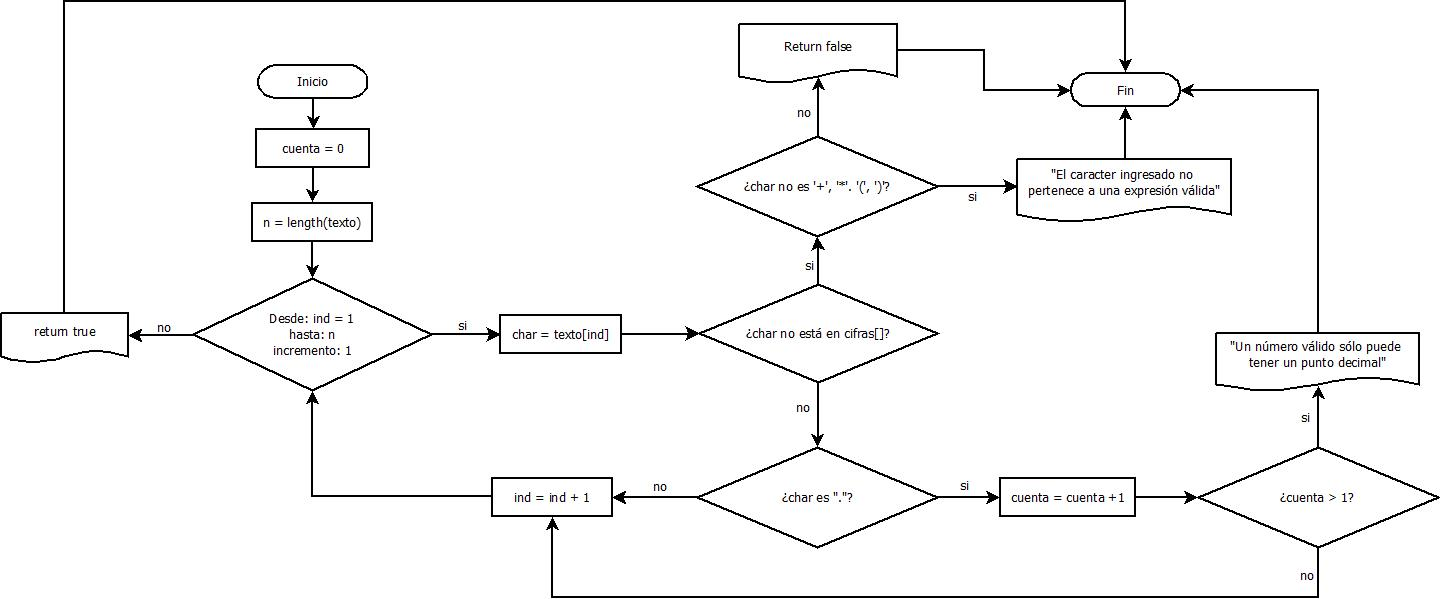
\includegraphics[scale=0.65]{Diagrama2.jpeg}
\end{landscape}

\subsection{Diagrama de flujo correspondiente a \texttt{function(eliminar\textunderscore paréntesis)}}
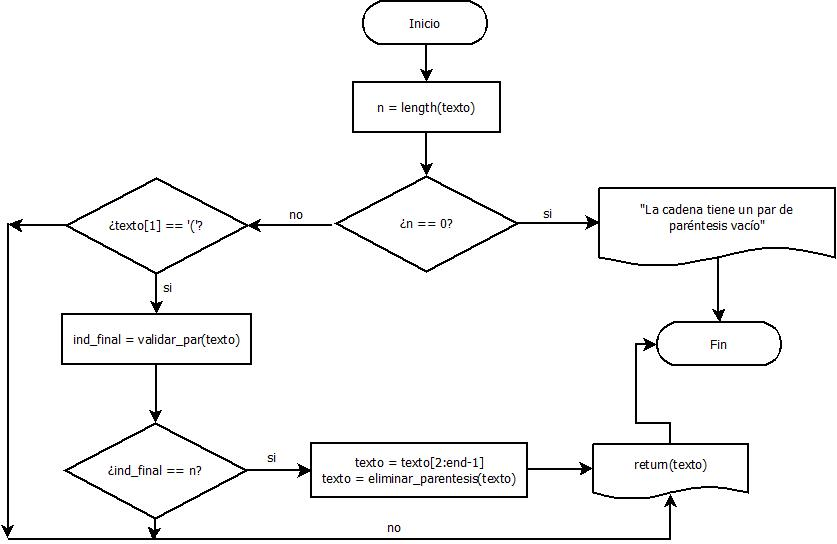
\includegraphics[scale=0.8]{Diagrama3.jpeg}

\begin{landscape}
    \subsection{Diagrama de flujo correspondiente a \texttt{function(validar\textunderscore par)}}\\
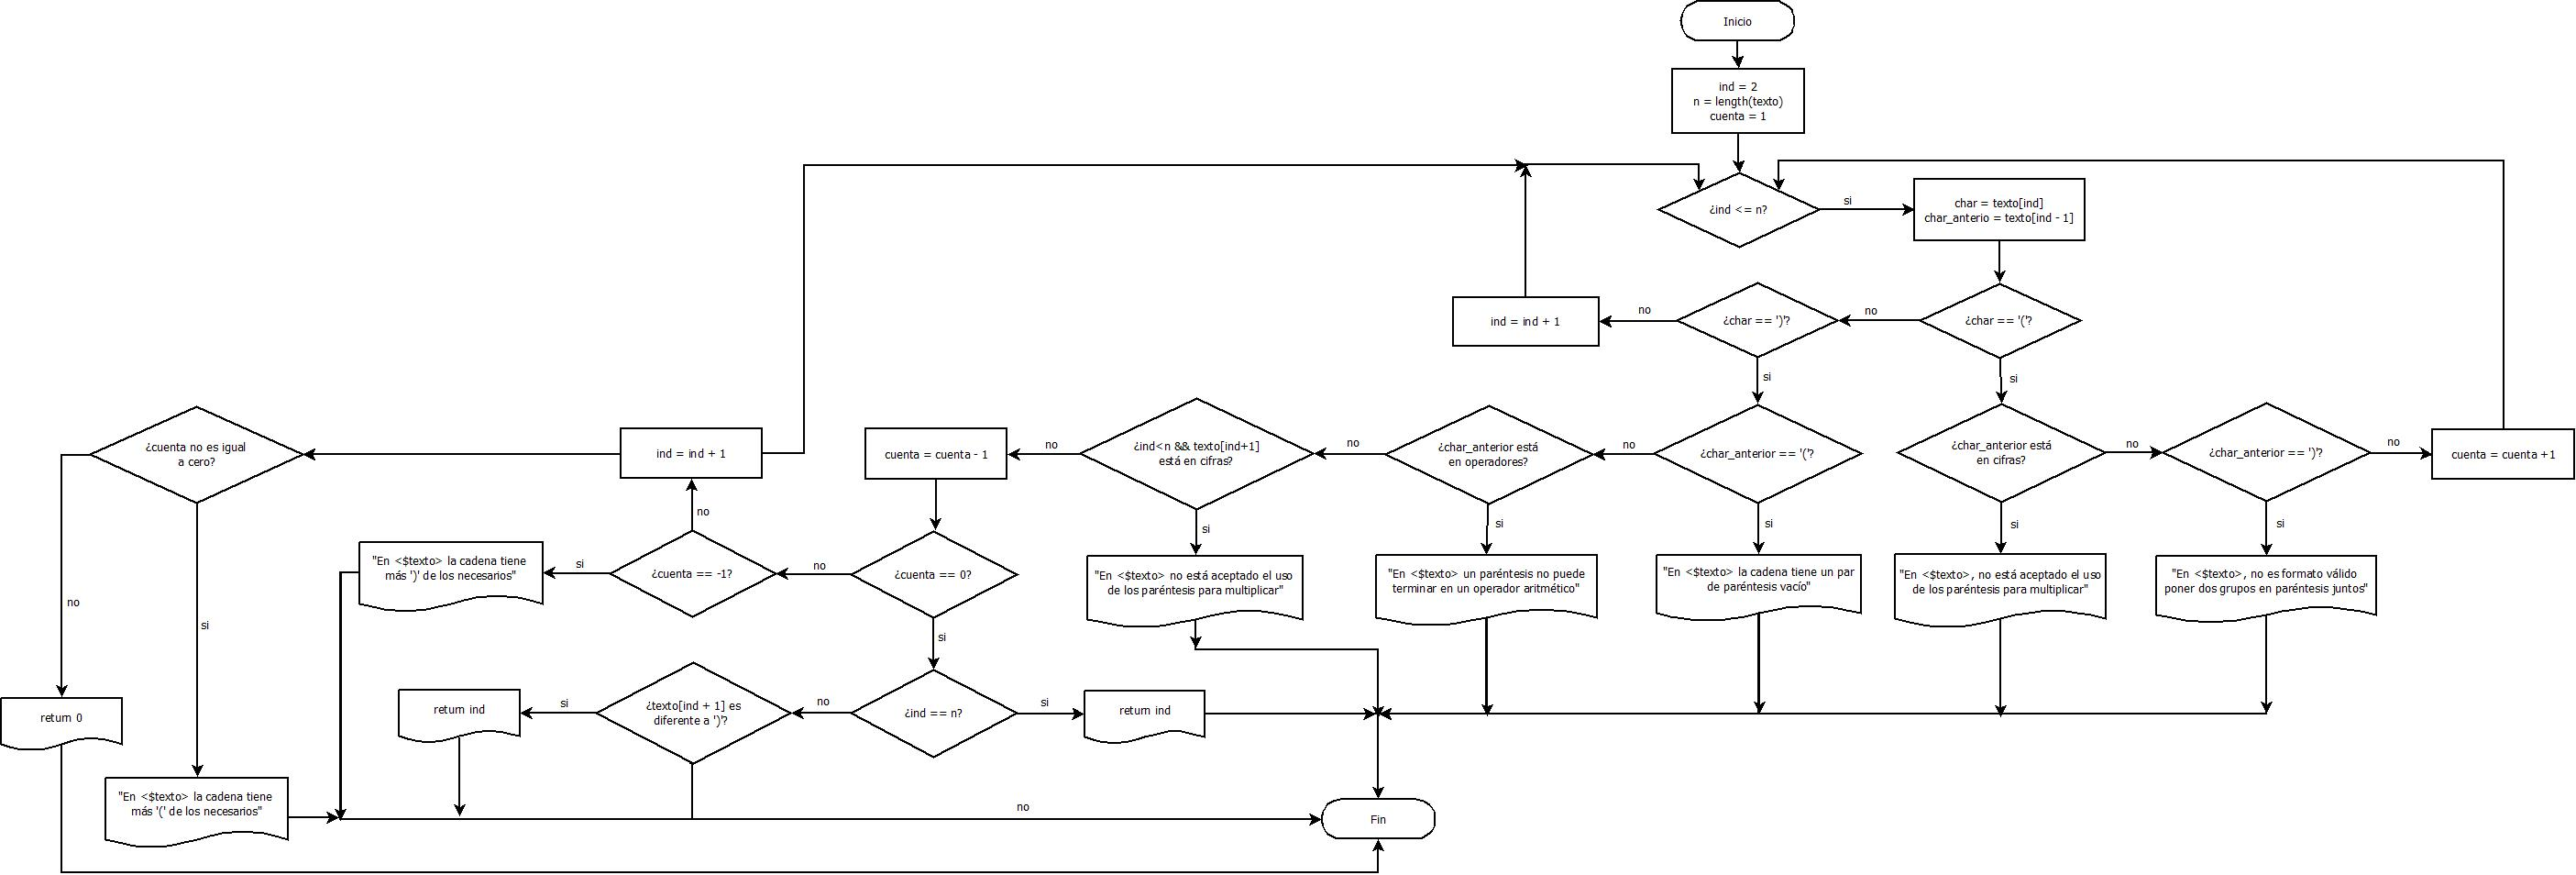
\includegraphics[scale=0.32]{Diagrama4.jpeg}
\end{landscape}

\subsection{Diagrama de flujo correspondiete a \texttt{function(encontrar\textunderscore operador)}}\\
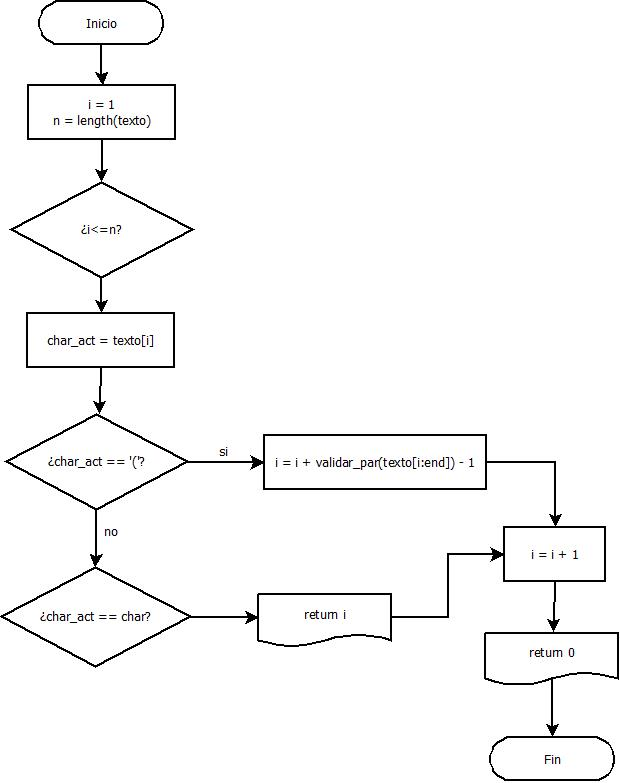
\includegraphics[scale=1]{Diagrama5.jpeg}

\begin{landscape}
    \subsection{Diagrama de flujo correspondiente a \texttt{function(calcular)}}\\
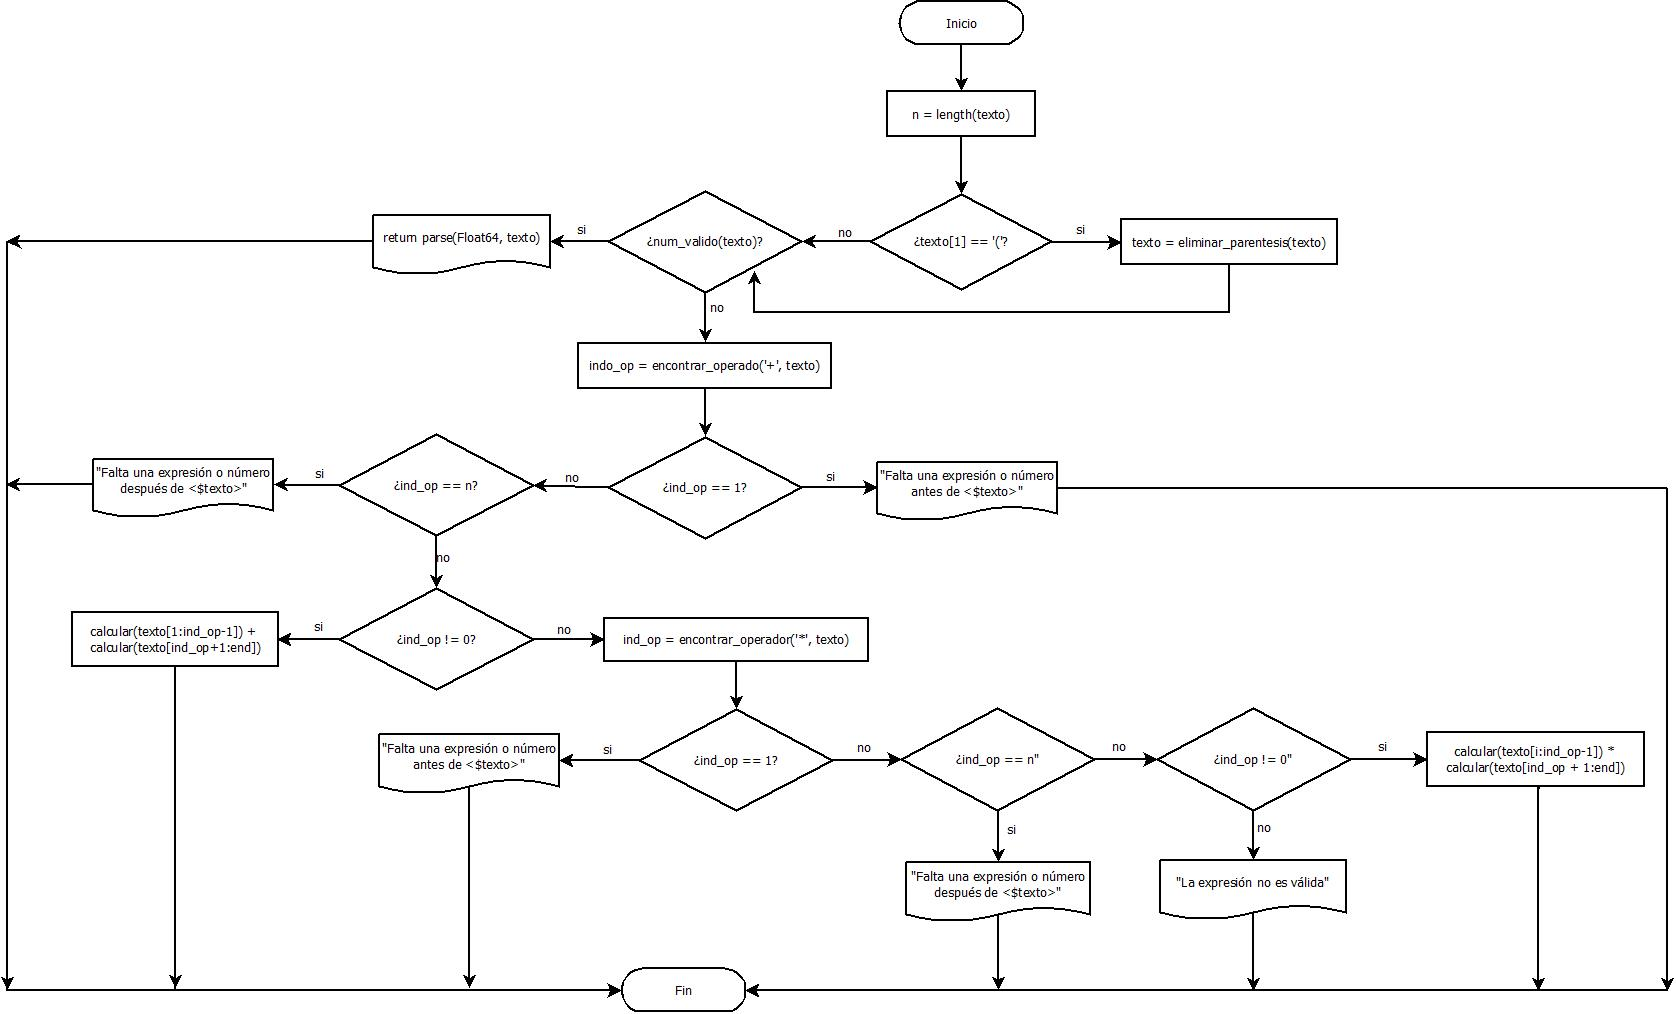
\includegraphics[scale=0.55]{Diagrama6.jpeg}
\end{landscape}

\subsection{Diagrama de flujo correspondiente a \texttt{function(main)}}\\
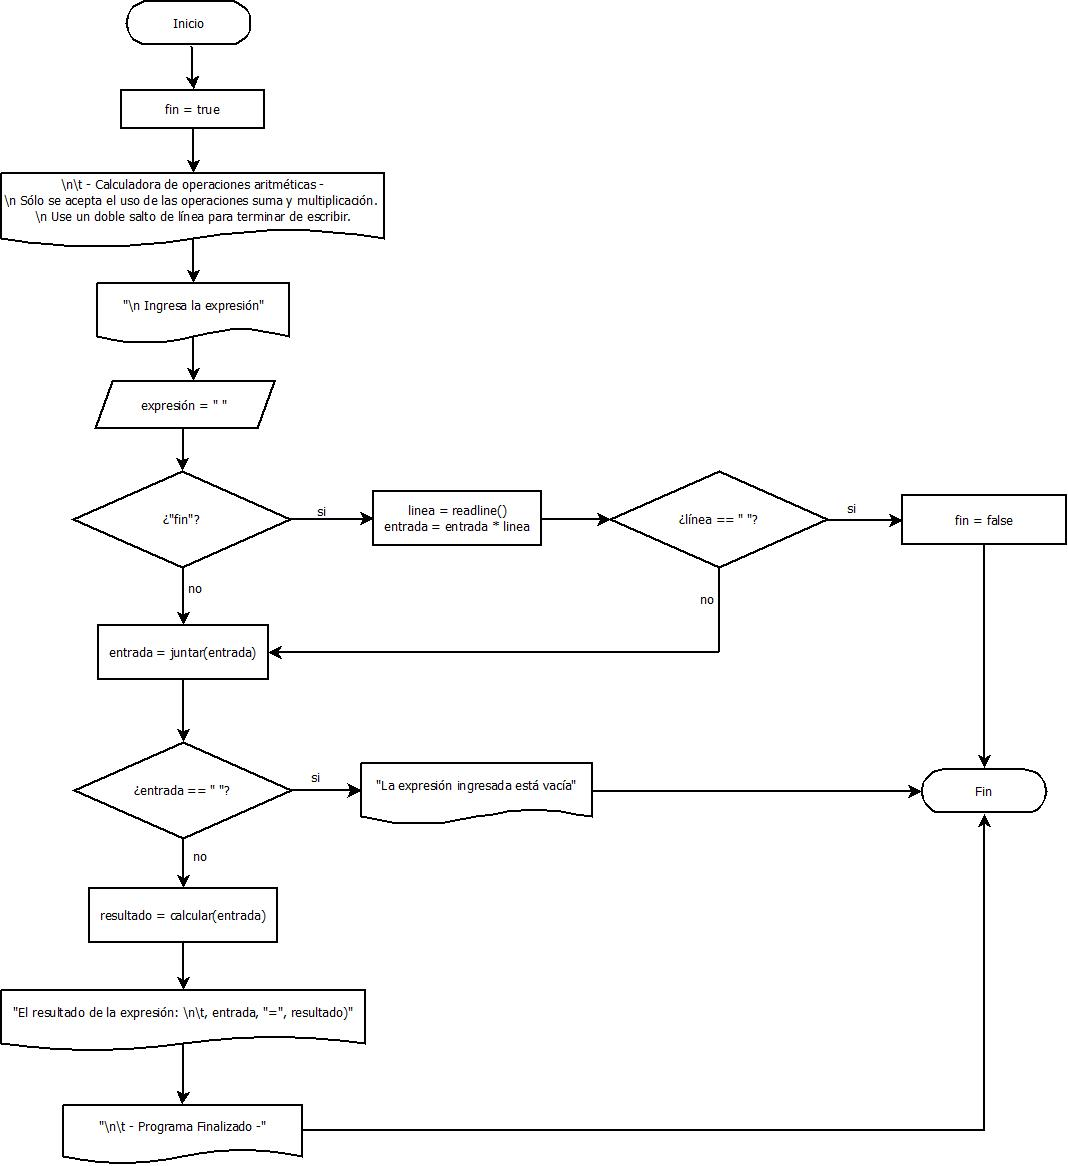
\includegraphics[scale=0.65]{Diagrama7.jpeg}

\newpage
\section{Instrucciones para utilizar el programa}
Para utilizar el interpretador aritmético, el usuario deberá seguir los siguientes pasos en su terminal:

\begin{enumerate}
    \item El usuario deberá navegar a la carpeta que contiene los archivos siguientes: \texttt{interpretador\textunderscore aritmético.jl} e \texttt{interprete\textunderscore aritmetico\textunderscore funciones.jl}.

    \item Una vez que se esté dentro de la carpeta, el usuario deberá ejecutar el comando \texttt{julia} para abrir la terminal de Julia.

    \item Deberá utilizar el comando \texttt{include("interpretador\textunderscore aritmetico.jl")}. Esto ejecutará la función del menú, que dará acceso a la función \texttt{calcular}.

    \item Dentro del menú, el usuario podrá ingresar una expresión aritmética. Esta expresión puede contener los siguientes símbolos: '(', ')', '+', '*', '.' y los números indo-arábigos. 

    \item Es importante mencionar que el usuario podrá añadir saltos de línea, espacios y tabuladores en cualquier parte de la expresión para mejorar su legibilidad. Para finalizar la entrada de texto, el usuario deberá utilizar un doble salto de línea. 

    \item Si la expresión no es válida desde el punto de vista aritmético, la función mostrará un mensaje de error que indicará el lugar en la expresión donde se encuentra el problema y la razón de la falla, para que de esta forma, el usuario tenga la oportunidad de modificar su expresión.\\
\end{enumerate}


\section{Porcentaje de contribución por integrante}
Ain Bolaños Cortés - \text{33.33\%} \\
Esteban Eguiarte Maldonado - \text{33.33\%} \\
Mariana Sánchez Esparza - \text{33.33\%}

\end{document}
